\documentclass[11pt,a4paper]{article}

\usepackage[utf8]{inputenc}
\usepackage[T1]{fontenc}
\usepackage[french]{babel}
\usepackage{lmodern}
\usepackage{geometry}
\usepackage{graphicx}
\usepackage{caption}
\usepackage{subcaption}
\usepackage{float}
\usepackage{booktabs}
\usepackage{amsmath}
\usepackage{amssymb}
\usepackage{hyperref}
\usepackage{xcolor}
\usepackage{url}

\geometry{margin=2.1cm}
\setlength{\parskip}{0.45em}
\setlength{\parindent}{0pt}
\captionsetup{font=small,labelfont=bf}
\hypersetup{colorlinks=true, linkcolor=black, citecolor=black, urlcolor=blue}
\definecolor{stormblue}{HTML}{0B1F33}
\definecolor{rainblue}{HTML}{1F77B4}
\definecolor{mistblue}{HTML}{EAF4FB}
\definecolor{slategray}{HTML}{5B6770}

\title{\textbf{Génération de champs de précipitations extrêmes en France par VAE et GAN}}
\author{Projet GenAI ENSAE}
\date{}

\begin{document}

\pagenumbering{gobble}
\hypersetup{pageanchor=false}
\begin{titlepage}
    \setlength{\fboxsep}{0pt}
    \thispagestyle{empty}
    \vspace*{0.2cm}

    \noindent\colorbox{stormblue}{%
        \begin{minipage}{0.98\textwidth}
            \vspace{0.18cm}
            \hspace{0.28cm}
            \begin{minipage}{0.90\textwidth}
            \color{white}
            \textbf{Projet GenAI ENSAE}
            \hfill
            Rapport de synthèse
            \end{minipage}
            \vspace{0.18cm}
        \end{minipage}
    }

    \vspace{1.0cm}

    \begin{center}
        {\color{rainblue}\rule{0.24\textwidth}{2.2pt}}\\[0.55cm]
        {\fontsize{26}{31}\selectfont\textbf{Génération de champs de précipitations extrêmes en France}}\\[0.3cm]
        {\fontsize{17}{21}\selectfont\color{slategray} Comparaison entre VAE, GAN et WGAN-GP}\\[0.45cm]
        {\large\color{slategray} Indice climatique Rx5day}
    \end{center}

    \vspace{0.65cm}

    \begin{center}
        \setlength{\fboxsep}{8pt}
        \fcolorbox{mistblue}{mistblue}{%
            \begin{minipage}{0.86\textwidth}
                \centering
                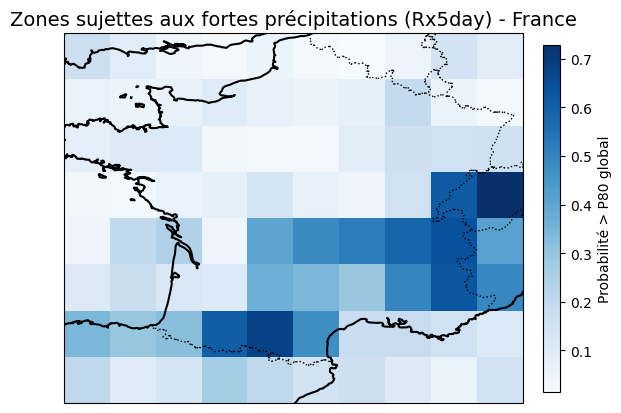
\includegraphics[width=0.64\linewidth]{../images/EDA/heavy_precipitation_probability_map.png}\\[-0.05cm]
                {\small\color{slategray} Probabilité empirique de fortes précipitations sur la zone française}
            \end{minipage}
        }
    \end{center}

    \vspace{0.75cm}

    \begin{center}
        \colorbox{mistblue}{\strut\hspace{0.55cm}\textbf{Analyse exploratoire}\hspace{0.55cm}}
        \hspace{0.35cm}
        \colorbox{mistblue}{\strut\hspace{0.55cm}\textbf{VAE}\hspace{0.55cm}}
        \hspace{0.35cm}
        \colorbox{mistblue}{\strut\hspace{0.55cm}\textbf{GAN / WGAN-GP}\hspace{0.55cm}}
    \end{center}

    \vfill

    \begin{center}
        \begin{minipage}{0.72\textwidth}
            \centering
            {\color{rainblue}\rule{\linewidth}{1pt}}\\[0.35cm]
            \begin{tabular}{@{}ll@{}}
                \textbf{Auteurs} & Nom Prénom 1 \\
                                  & Nom Prénom 2 \\
                                  & Nom Prénom 3 \\[0.25cm]
                \textbf{Encadrant} & Nom Prénom \\
            \end{tabular}\\[0.35cm]
            {\color{slategray}\small 27 avril 2026}
        \end{minipage}
    \end{center}
\end{titlepage}
\clearpage
\pagenumbering{arabic}
\hypersetup{pageanchor=true}

\section{Introduction}

Les épisodes de précipitations extrêmes jouent un rôle central dans l'évaluation des risques climatiques. Dans ce travail, on s'intéresse à l'indice Rx5day, défini comme le maximum de précipitation cumulé sur cinq jours consécutifs. Cet indicateur est pertinent car il résume des événements intenses sur une échelle temporelle suffisamment longue pour être liée à des impacts hydrologiques majeurs.

L'objectif de ce projet est d'évaluer dans quelle mesure des modèles génératifs profonds (VAE, GAN, WGAN-GP) peuvent agir comme des émulateurs climatiques rapides pour contourner la lourdeur des Modèles de Circulation Générale (GCM). Le défi est d'apprendre la structure spatiale complexe de ces champs et de produire de nouveaux scénarios plausibles. Un modèle utile doit reproduire les contrastes régionaux, la forte asymétrie des distributions, et les corrélations spatiales locales. 

Le rapport caractérise d'abord les données, puis interprète les résultats des réseaux de neurones en insistant sur la stabilité d'apprentissage et la qualité spatiale des cartes générées.

\section{Données et prétraitement}

La base de données provient du Climate Data Store via les projections globales CMIP6 \cite{copernicus_cmip6_extreme_indices, eyring2016cmip6}. On exploite la variable \texttt{rx5dayETCCDI}, restreinte à une fenêtre spatiale recouvrant la France métropolitaine ($[41^\circ N, 52^\circ N] \times [-5^\circ E, 9^\circ E]$). Chaque observation est représentée comme une petite image de taille $8 \times 10$ pixels avec un canal unique.

Les valeurs subissent une normalisation par \textit{min-max scaling} pour contraindre l'intervalle dans $[0, 1]$. Bien qu'indispensable pour utiliser des fonctions d'activation sigmoïdes en sortie des réseaux, cette transformation introduit une limitation climatologique majeure. Les précipitations extrêmes suivant des lois à queue lourde, le scaling linéaire écrase la vaste majorité des valeurs modérées près de zéro. Cette asymétrie complique la tâche des modèles, rendant la modélisation fine des gradients de tempêtes particulièrement difficile.

\section{Analyse exploratoire}

L'analyse exploratoire des champs $8 \times 10$ pixels met en évidence trois propriétés climatologiques fondamentales : une saisonnalité prononcée, une hétérogénéité spatiale structurelle, et une corrélation locale. Ces éléments constituent la "vérité terrain" que les réseaux antagonistes ou variationnels devront émuler.

\begin{figure}[H]
    \centering
    \begin{subfigure}{0.48\textwidth}
        \centering
        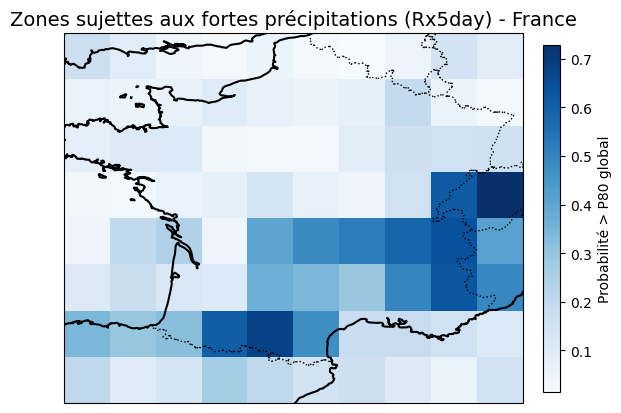
\includegraphics[width=\textwidth]{../images/EDA/heavy_precipitation_probability_map.png}
        \caption{Probabilité de dépassement (P80)}
    \end{subfigure}
    \hfill
    \begin{subfigure}{0.48\textwidth}
        \centering
        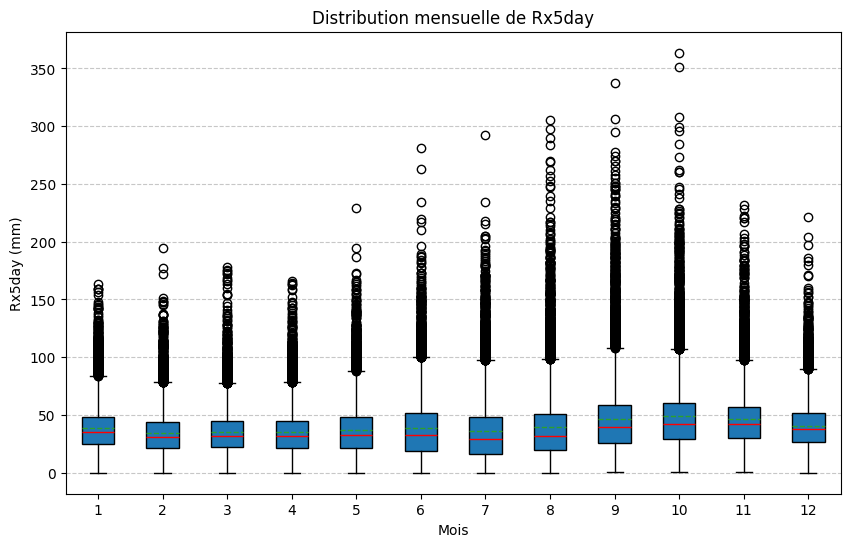
\includegraphics[width=\textwidth]{../images/EDA/monthly_rx5day_boxplot.png}
        \caption{Distribution mensuelle}
    \end{subfigure}
    \caption{Caractéristiques des fortes précipitations (Rx5day).}
    \label{fig:eda-combined}
\end{figure}

La figure \ref{fig:eda-combined}a montre que les fortes précipitations ne sont pas un bruit blanc uniformément réparti sur le territoire. Les probabilités de dépassement du 80e percentile sont significativement plus élevées dans des zones géographiques précises, notamment au sud-est (influence méditerranéenne) et sur les reliefs. La figure \ref{fig:eda-combined}b indique quant à elle une variabilité mensuelle nette. Les distributions statistiques des intensités sont fortement asymétriques avec des queues droites prononcées en automne et en hiver. Bien que les modèles (VAE et GAN) soient entraînés sur l'ensemble des observations temporelles de manière agnostique (sans recevoir le mois en entrée), un modèle pertinent devra implicitement encoder cette saisonnalité dans son espace latent pour générer une carte réaliste.

\begin{figure}[H]
    \centering
    \begin{subfigure}{0.48\textwidth}
        \centering
        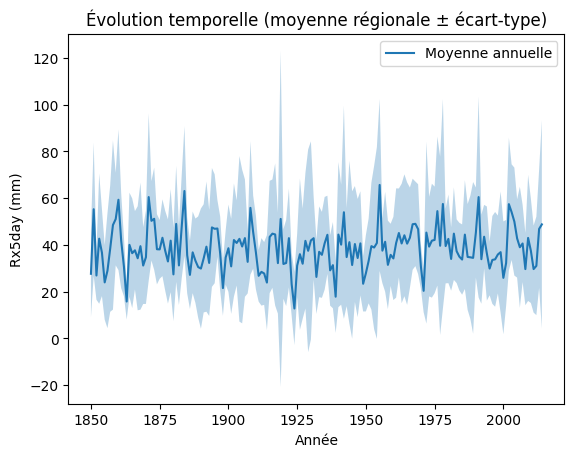
\includegraphics[width=0.8\textwidth]{../images/EDA/annual_mean_time_series.png}
        \caption{Moyenne régionale annuelle}
    \end{subfigure}
    \hfill
    \begin{subfigure}{0.48\textwidth}
        \centering
        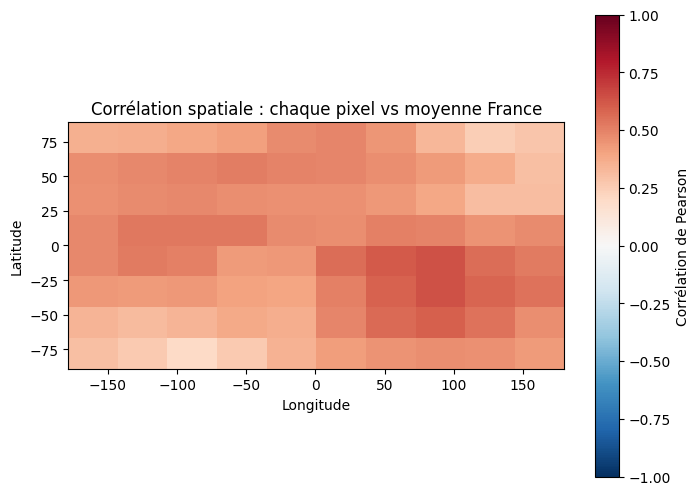
\includegraphics[width=\textwidth]{../images/EDA/spatial_correlation_map.png}
        \caption{Corrélation spatiale locale}
    \end{subfigure}
    \caption{Variabilité temporelle et structure spatiale des champs Rx5day.}
    \label{fig:eda-time-space}
\end{figure}

La carte de corrélation spatiale (Fig. \ref{fig:eda-time-space}b) démontre que les pixels voisins réagissent de manière cohérente, justifiant pleinement le choix d'architectures basées sur les Réseaux de Neurones Convolutifs (CNN) plutôt que des perceptrons multicouches complets. Les filtres convolutifs pourront ainsi balayer la carte pour détecter les gradients de cellules orageuses.

Pour aller plus loin, une segmentation non supervisée par l'algorithme \textit{k-means} appliquée sur l'axe des pixels (k=2, score de silhouette moyen de 0.355) a été réalisée (voir figures \ref{fig:kmeans-seg} et \ref{fig:kmeans-dist}). Cette partition suggère l'existence de deux grandes zones climatiques comportementales : une vaste zone sous influence océanique atlantique (où les précipitations maximales sont fréquentes mais d'intensité modérée) et une zone plus restreinte méditerranéenne et montagneuse (sujette à des événements sporadiques mais d'une violence extrême, tels que les épisodes cévenols). Cette double dualité impose aux modèles génératifs de ne pas apprendre une "texture" unique pour toute l'image, mais bien d'apprendre à déclencher des motifs locaux d'intensité variable selon les coordonnées spatiales.

\begin{figure}[H]
    \centering
    \begin{subfigure}{0.48\textwidth}
        \centering
        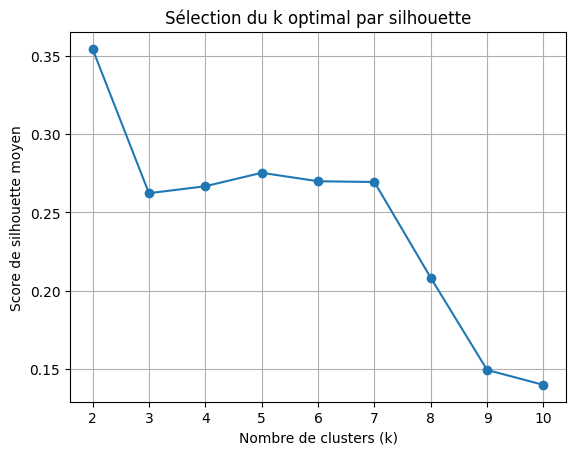
\includegraphics[width=\textwidth]{../images/EDA/cluster_silhouette_curve.png}
        \caption{Choix du nombre de clusters}
    \end{subfigure}
    \hfill
    \begin{subfigure}{0.48\textwidth}
        \centering
        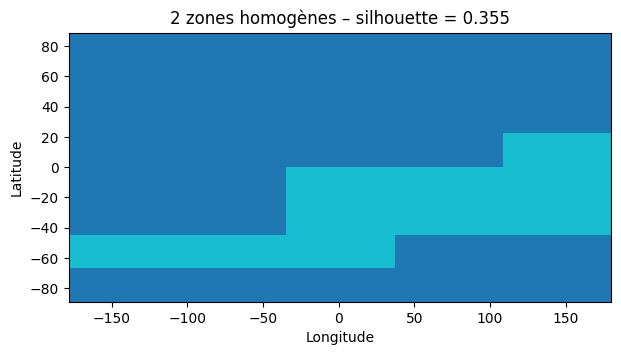
\includegraphics[width=\textwidth]{../images/EDA/homogeneous_precipitation_zones.png}
        \caption{Zones homogènes}
    \end{subfigure}
    \caption{Segmentation spatiale des précipitations extrêmes (k-means).}
    \label{fig:kmeans-seg}
\end{figure}

\begin{figure}[H]
    \centering
    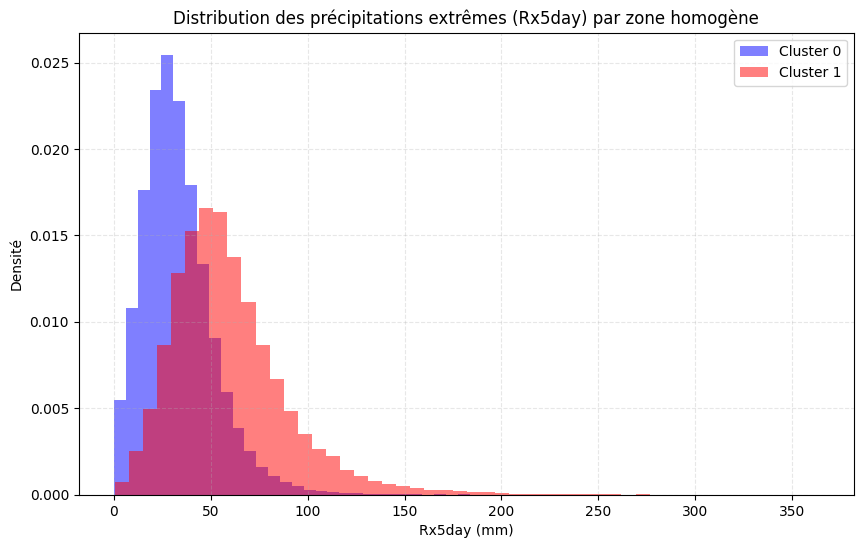
\includegraphics[width=0.75\textwidth]{../images/EDA/cluster_precipitation_distribution.png}
    \caption{Distribution des précipitations extrêmes (Rx5day) par zone homogène.}
    \label{fig:kmeans-dist}
\end{figure}

\section{Autoencodeur variationnel (VAE)}

Le VAE \cite{kingma2014vae} aborde la génération par une approche probabiliste explicite. Il compresse chaque carte Rx5day de $8 \times 10$ pixels dans un espace latent de dimension réduite (fixée ici à 8), forçant le réseau à extraire les caractéristiques macroscopiques essentielles des systèmes pluvieux. L'encodeur cartographie l'image vers une distribution gaussienne (définie par les vecteurs $z_{\mu}$ et $z_{\log\sigma^2}$), à partir de laquelle un vecteur $z$ est échantillonné puis traité par le décodeur. Les deux blocs reposent sur des architectures convolutives simples mais efficaces (deux couches convolutives d'encodage, suivies de couches denses, et des convolutions transposées pour le décodage).

L'entraînement est guidé par l'optimisation de la borne inférieure de l'évidence (ELBO), qui se traduit par une fonction de perte combinant un terme de reconstruction (ici, la Binary Cross-Entropy - BCE, adaptée aux valeurs dans $[0, 1]$) et un terme de régularisation (la divergence de Kullback-Leibler - KL) :
\[
\mathcal{L} = \lambda_{\mathrm{rec}}\mathcal{L}_{\mathrm{BCE}} + \lambda_{\mathrm{KL}}D_{\mathrm{KL}}(q(z|x)\Vert p(z)).
\]

Une recherche approfondie d'hyperparamètres a été menée sur le notebook, révélant la configuration optimale détaillée dans le tableau \ref{tab:vae-params}.

\begin{table}[H]
    \centering
    \caption{Configuration optimale de l'Autoencodeur Variationnel.}
    \label{tab:vae-params}
    \small
    \begin{tabular}{lc}
        \toprule
        \textbf{Hyperparamètre} & \textbf{Valeur optimale} \\
        \midrule
        Dimension latente (\texttt{latent\_dim}) & 8 \\
        Poids divergence KL (\texttt{kl\_weight}) & 0.005 \\
        Taux d'apprentissage (\texttt{learning\_rate}) & 0.001 \\
        Taille de batch (\texttt{batch\_size}) & 16 \\
        \midrule
        \textbf{Perte finale (Loss)} & $\approx 421.9$ \\
        \bottomrule
    \end{tabular}
\end{table} 

Deux points théoriques majeurs ressortent de cette recherche :

Premièrement, le poids $\lambda_{\mathrm{KL}}$ optimal est très faible (0.005). Ce déséquilibre volontaire sacrifie un peu la régularité mathématique de la distribution latente au profit d'une reconstruction fidèle (BCE). Si $\lambda_{\mathrm{KL}}$ était trop élevé, le modèle souffrirait de "posterior collapse", se contentant de produire la carte moyenne de France indépendamment du vecteur latent, ce qui est fatal pour l'étude des extrêmes locaux.

Deuxièmement, la \textbf{taille de batch} s'est avérée être le facteur de bascule critique. Le passage d'un \texttt{batch\_size = 16} à 32 provoque systématiquement un doublement de la perte (stagnant autour de 850). L'explication réside dans la rareté des extrêmes : dans un grand batch, les gradients rétropropagés par les rares pixels de fortes tempêtes sont noyés et annulés par la masse des gradients des pixels "secs" ou modérés. Le modèle converge alors vers un minimum local sûr (prédire peu de pluie partout). Un batch réduit (16) injecte le bruit stochastique nécessaire à la descente de gradient pour préserver l'impact des anomalies pluviométriques.

\begin{figure}[H]
    \centering
    \begin{subfigure}{0.37\textwidth}
        \centering
        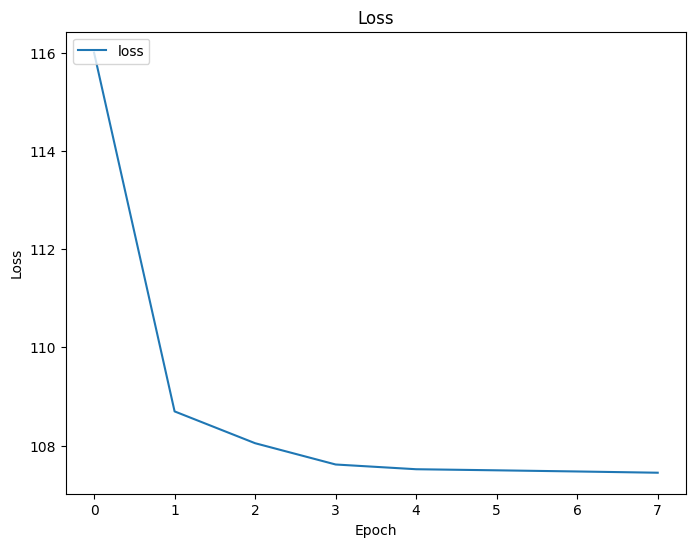
\includegraphics[width=\textwidth]{../images/VAE/vae_training_loss_curve.png}
        \caption{Perte d'entraînement}
    \end{subfigure}
    \hfill
    \begin{subfigure}{0.58\textwidth}
        \centering
        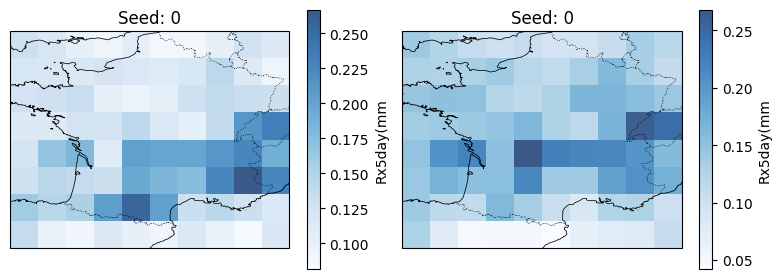
\includegraphics[width=\textwidth]{../images/VAE/vae_decoded_random_maps_seed_zero.png}
        \caption{Cartes générées depuis l'espace latent}
    \end{subfigure}
    \caption{Dynamique d'apprentissage et génération synthétique par VAE.}
    \label{fig:vae-main}
\end{figure}

L'évaluation visuelle des cartes générées (Fig. \ref{fig:vae-main}b) montre que le VAE est capable de restituer des positionnements géographiques plausibles, respectant les zones climatiques évoquées plus tôt. Cependant, la nature même de la fonction de perte (qui pénalise l'erreur moyenne) contraint le VAE à produire des champs lissés et floutés, manquant de la netteté et de l'abrupté spatiale caractéristiques des véritables orages extrêmes.

L'analyse de l'espace latent (cf. figures en annexe) apporte une clé de lecture supplémentaire. En projetant les vecteurs latents et en les colorant par saison, on observe un fort chevauchement. Ce phénomène, loin d'être un échec du réseau, s'explique climatiquement : l'indice Rx5day ciblant les extrêmes les plus intenses, des événements survenant en automne et en été peuvent partager des signatures synoptiques ou des textures spatiales très similaires qui sont logiquement groupées par l'encodeur. Bien que certaines directions latentes captent un biais saisonnier, aucune frontière linéaire simple ne permet d'isoler mécaniquement les saisons.

\section{Approches adversariales : GAN et WGAN-GP}

Pour pallier le problème de lissure du VAE, les approches adversariales (GAN) ont été explorées. Ces modèles \cite{goodfellow2014gan} apprennent à cartographier un bruit aléatoire vers la distribution des données réelles par un jeu à somme nulle entre un Générateur ($G$) et un Discriminateur ($D$), sans jamais calculer de distance pixel-à-pixel avec une image de référence. Les formulations des deux variantes étudiées sont résumées dans le tableau \ref{tab:gan-wgan-summary}.

\begin{table}[H]
    \centering
    \caption{Résumé mathématique et comportemental des modèles adversariaux implémentés.}
    \label{tab:gan-wgan-summary}
    \small
    \begin{tabular}{p{0.18\textwidth}p{0.45\textwidth}p{0.28\textwidth}}
        \toprule
        Modèle & Fonction objectif principale & Comportement empirique \\
        \midrule
        GAN classique & $\min_G \max_D \mathbb{E}_x[\log D(x)] + \mathbb{E}_z[\log(1-D(G(z)))]$ & Cartes hautement contrastées. Dynamique minimax instable ("mode collapse" fréquent). \\
        WGAN-GP \cite{gulrajani2017wgangp} & $\mathcal{L}_D= \mathbb{E}_z[f_w(G(z))] -\mathbb{E}_x[f_w(x)] +\lambda GP$ & Gradients de perte continus. Stabilité améliorée, mais présence persistante d'artefacts. \\
        \bottomrule
    \end{tabular}
\end{table}

Les architectures neuronales utilisées ici sont très compactes (pour permettre un apprentissage local sur CPU) : le générateur empile des couches denses, des \textit{upsampling} et des convolutions, tandis que le discriminateur agit comme un extracteur de caractéristiques avec des convolutions, des activations \textit{LeakyReLU} et du \textit{dropout} pour freiner le surapprentissage.

\begin{figure}[H]
    \centering
    \begin{subfigure}{0.48\textwidth}
        \centering
        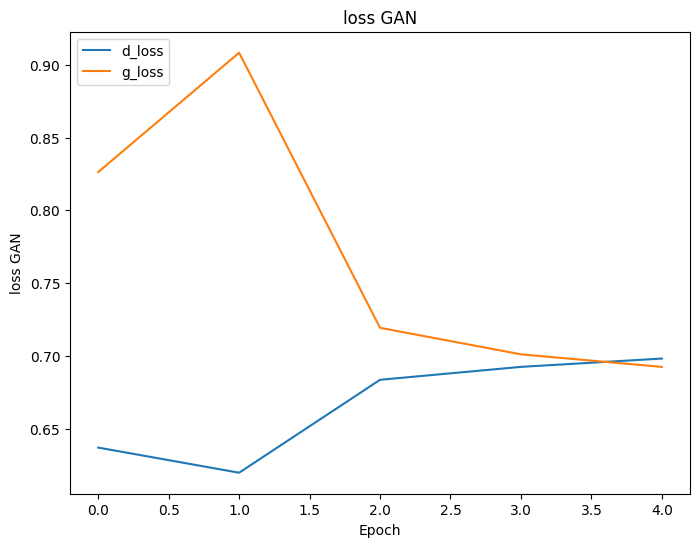
\includegraphics[width=\textwidth]{../images/GAN/gan_training_loss_curve.png}
        \caption{Pertes du GAN classique}
    \end{subfigure}
    \hfill
    \begin{subfigure}{0.48\textwidth}
        \centering
        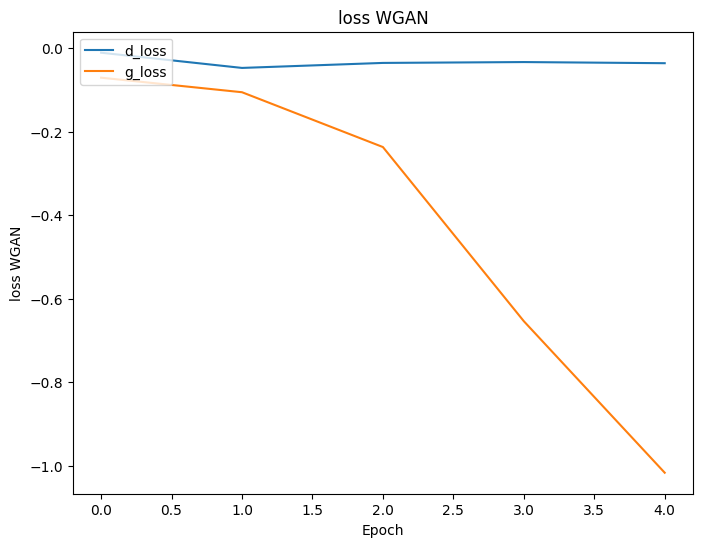
\includegraphics[width=\textwidth]{../images/GAN/wgan_training_loss_curve.png}
        \caption{Pertes du WGAN-GP}
    \end{subfigure}
    \caption{Évolution des pertes adversariales au cours de l'entraînement.}
    \label{fig:gan-loss}
\end{figure}

\begin{figure}[H]
    \centering
    \begin{subfigure}{0.75\textwidth}
        \centering
        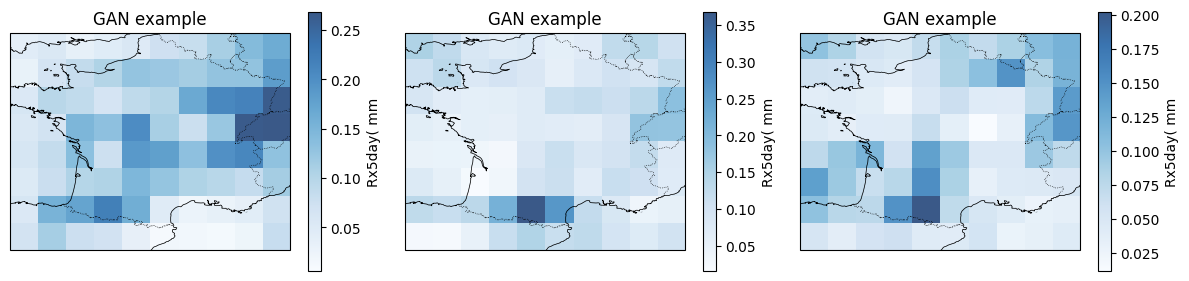
\includegraphics[width=\textwidth]{../images/GAN/gan_final_generated_precipitation_maps.png}
        \caption{Exemples GAN classique}
    \end{subfigure}
    
    \vspace{0.4cm}
    
    \begin{subfigure}{0.75\textwidth}
        \centering
        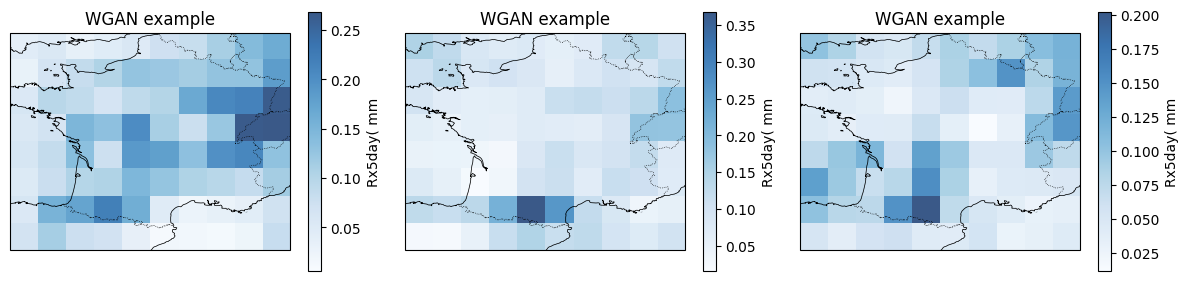
\includegraphics[width=\textwidth]{../images/GAN/wgan_final_generated_precipitation_maps.png}
        \caption{Exemples WGAN-GP}
    \end{subfigure}
    \caption{Champs synthétiques générés par les modèles adversariaux après entraînement complet.}
    \label{fig:gan-samples}
\end{figure}

Visuellement (Fig. \ref{fig:gan-samples}), la différence avec le VAE est frappante. Les champs générés par les GANs sont nettement plus abrupts, présentant des pics d'intensité entourés de gradients forts, ce qui représente une propriété hautement désirable pour la modélisation de catastrophes locales.

Cependant, l'entraînement de ces modèles s'est révélé particulièrement ardu. Le problème fondamental des GANs classiques dans ce contexte météorologique réside dans la nature fortement asymétrique et parcimonieuse des données. Contrairement à des visages ou des paysages naturels qui contiennent de l'information sur chaque pixel, les champs Rx5day sont dominés par de vastes zones de précipitations très faibles, ponctuées de quelques pixels extrêmes. Cette structure crée un piège fatal : le Discriminateur probabiliste apprend extrêmement vite à repérer les erreurs de sparsité (par exemple, si le générateur met un peu de pluie "floue" là où il ne devrait y avoir rien), rejetant en bloc les propositions du générateur et annulant le flux de gradient utile.

Le WGAN-GP apporte une réponse mathématique élégante en remplaçant la métrique de Jensen-Shannon par la distance de Wasserstein (Earth Mover's Distance). Le Discriminateur devient un "Critique" lipschitzien (contraint par la pénalité de gradient $GP$) qui quantifie le "coût de transport" pour transformer la distribution générée en distribution réelle. Cela garantit un retour de gradient lisse et utile même lorsque les champs générés sont très mauvais. Bien que les courbes de perte du WGAN-GP soient théoriquement plus saines, les images finales (Fig. \ref{fig:gan-samples}b) présentent encore des artefacts géométriques ("checkerboard artifacts"). Ces défauts en damier sont souvent le symptôme de déconvolutions mal calibrées (taille de filtre non divisible par le pas) s'exprimant sur des espaces très contraignants ($8 \times 10$).

\section{Discussion et conclusion}

La génération stochastique de champs d'extrêmes climatiques (Rx5day) par des réseaux de neurones profonds est un défi d'émulation singulier. Un algorithme performant ne doit pas seulement tromper l'œil humain, mais il doit reproduire une physique sous-jacente faite de distributions fortement asymétriques à queue lourde, de contrastes régionaux clivés, et de corrélations spatiales locales.

L'étude comparative menée dans ce rapport permet de trancher sur les forces en présence. Le \textbf{VAE} s'impose sans conteste comme le modèle le plus robuste sur le plan expérimental. Il garantit une convergence stable et offre l'accès direct à un espace latent continu, propice à l'interpolation entre scénarios climatiques. L'analyse a notamment mis en lumière que la modélisation des extrêmes avec ce modèle exigeait un \textit{batch size} réduit (16) pour conserver la trace stochastique des tempêtes intenses et éviter un effondrement global vers la moyenne. Toutefois, contraint par sa nature variationnelle, le VAE tend systématiquement à adoucir l'intensité spatiale des événements, ce qui pose une limite fondamentale pour son utilisation directe en tant que générateur de stress-tests hydrologiques.

À l'inverse, les approches adversariales (\textbf{GAN} et \textbf{WGAN-GP}) détiennent le potentiel structurel de générer des gradients de pluie brutaux et réalistes. Néanmoins, leur mise en pratique se heurte de plein fouet à la rareté statistique des signaux climatiques forts. La sparsité des champs de précipitation provoque des dynamiques d'entraînement instables, que seule la métrique de Wasserstein parvient à partiellement dompter.

L'une des limitations actuelles de l'étude est son évaluation essentiellement qualitative et visuelle (les courbes de perte adversarial n'étant pas corrélées à une qualité métrique absolue). Pour transformer ces prototypes en outils opérationnels de simulation climatique, de futurs travaux devront impérativement intégrer des métriques quantitatives d'évaluation spécialisées : l'application de la distance de Wasserstein empirique sur les histogrammes d'intensité, le calcul de la Root Mean Square Error (RMSE) sur la matrice de covariance spatiale, ou l'utilisation d'une Fréchet Inception Distance (FID) recalibrée pour des canaux climatiques uniques. 

En conclusion, la modélisation d'extrêmes climatiques appelle une architecture hybride. La combinaison de la stabilité encodée d'un VAE avec l'affûtage local d'un critique WGAN (modèles de type VAE-GAN), le tout conditionné par un vecteur forçant saisonnier ou géographique, représente la perspective la plus prometteuse pour concilier la robustesse de l'apprentissage et le réalisme physique des cataclysmes simulés.

\clearpage
\begin{thebibliography}{9}

\bibitem{copernicus_cmip6_extreme_indices}
Copernicus Climate Change Service, Climate Data Store.
\textit{Climate extreme indices and heat stress indicators derived from CMIP6 global climate projections}.
DOI: \href{https://doi.org/10.24381/cds.776e08bd}{10.24381/cds.776e08bd}.
Publication : 14 janvier 2022 ; mise à jour : 31 janvier 2025.
URL : \url{https://cds.climate.copernicus.eu/datasets/sis-extreme-indices-cmip6}.

\bibitem{eyring2016cmip6}
Eyring, V., Bony, S., Meehl, G. A., Senior, C. A., Stevens, B., Stouffer, R. J. et Taylor, K. E. (2016).
\textit{Overview of the Coupled Model Intercomparison Project Phase 6 (CMIP6) experimental design and organization}.
Geoscientific Model Development, 9, 1937--1958.

\bibitem{kingma2014vae}
Kingma, D. P. et Welling, M. (2014).
\textit{Auto-Encoding Variational Bayes}.
International Conference on Learning Representations.

\bibitem{goodfellow2014gan}
Goodfellow, I., Pouget-Abadie, J., Mirza, M., Xu, B., Warde-Farley, D., Ozair, S., Courville, A. et Bengio, Y. (2014).
\textit{Generative Adversarial Nets}.
Advances in Neural Information Processing Systems.

\bibitem{gulrajani2017wgangp}
Gulrajani, I., Ahmed, F., Arjovsky, M., Dumoulin, V. et Courville, A. (2017).
\textit{Improved Training of Wasserstein GANs}.
Advances in Neural Information Processing Systems.

\end{thebibliography}

\appendix
\clearpage
\section{Analyses complémentaires}

\begin{figure}[H]
    \centering
    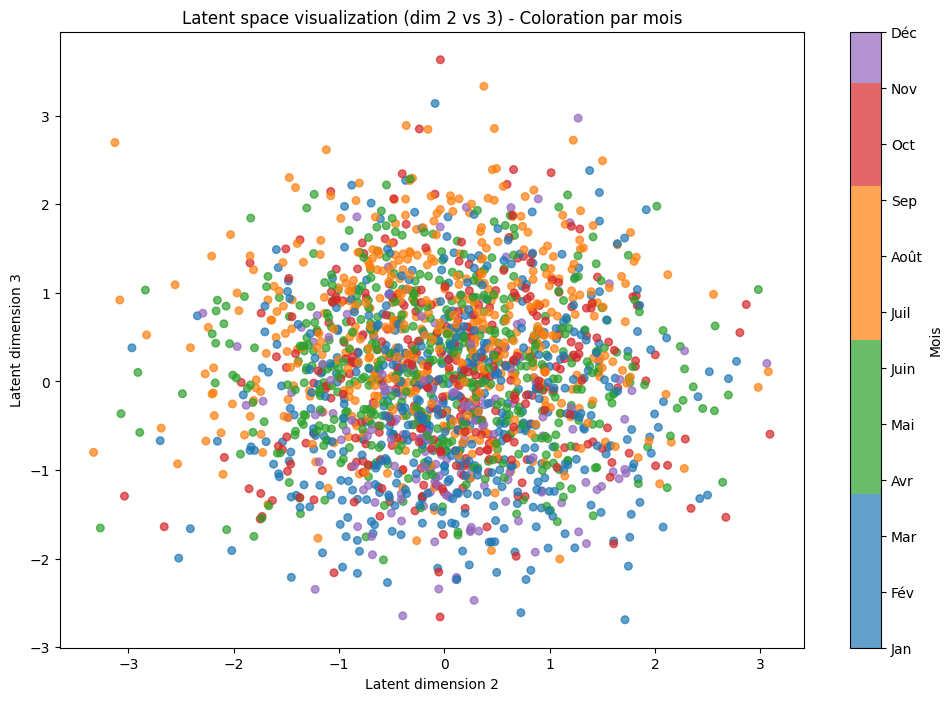
\includegraphics[width=0.7\textwidth]{../images/VAE/vae_latent_space_by_season.png}
    \caption{Projection de l'espace latent du VAE colorée par saison.}
\end{figure}

\begin{figure}[H]
    \centering
    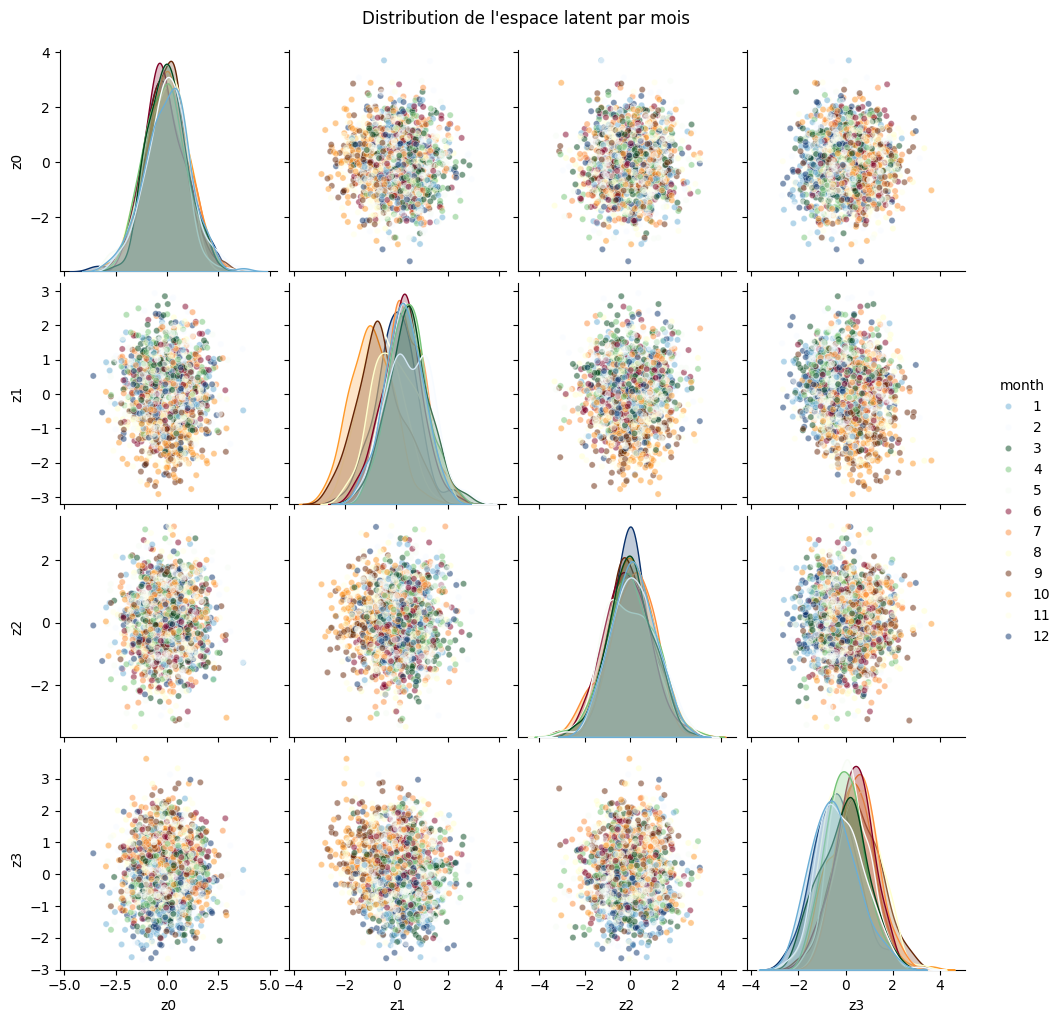
\includegraphics[width=0.82\textwidth]{../images/VAE/vae_latent_pairplot_by_season.png}
    \caption{Relations deux à deux entre dimensions latentes du VAE, colorées par saison.}
\end{figure}

\begin{figure}[H]
    \centering
    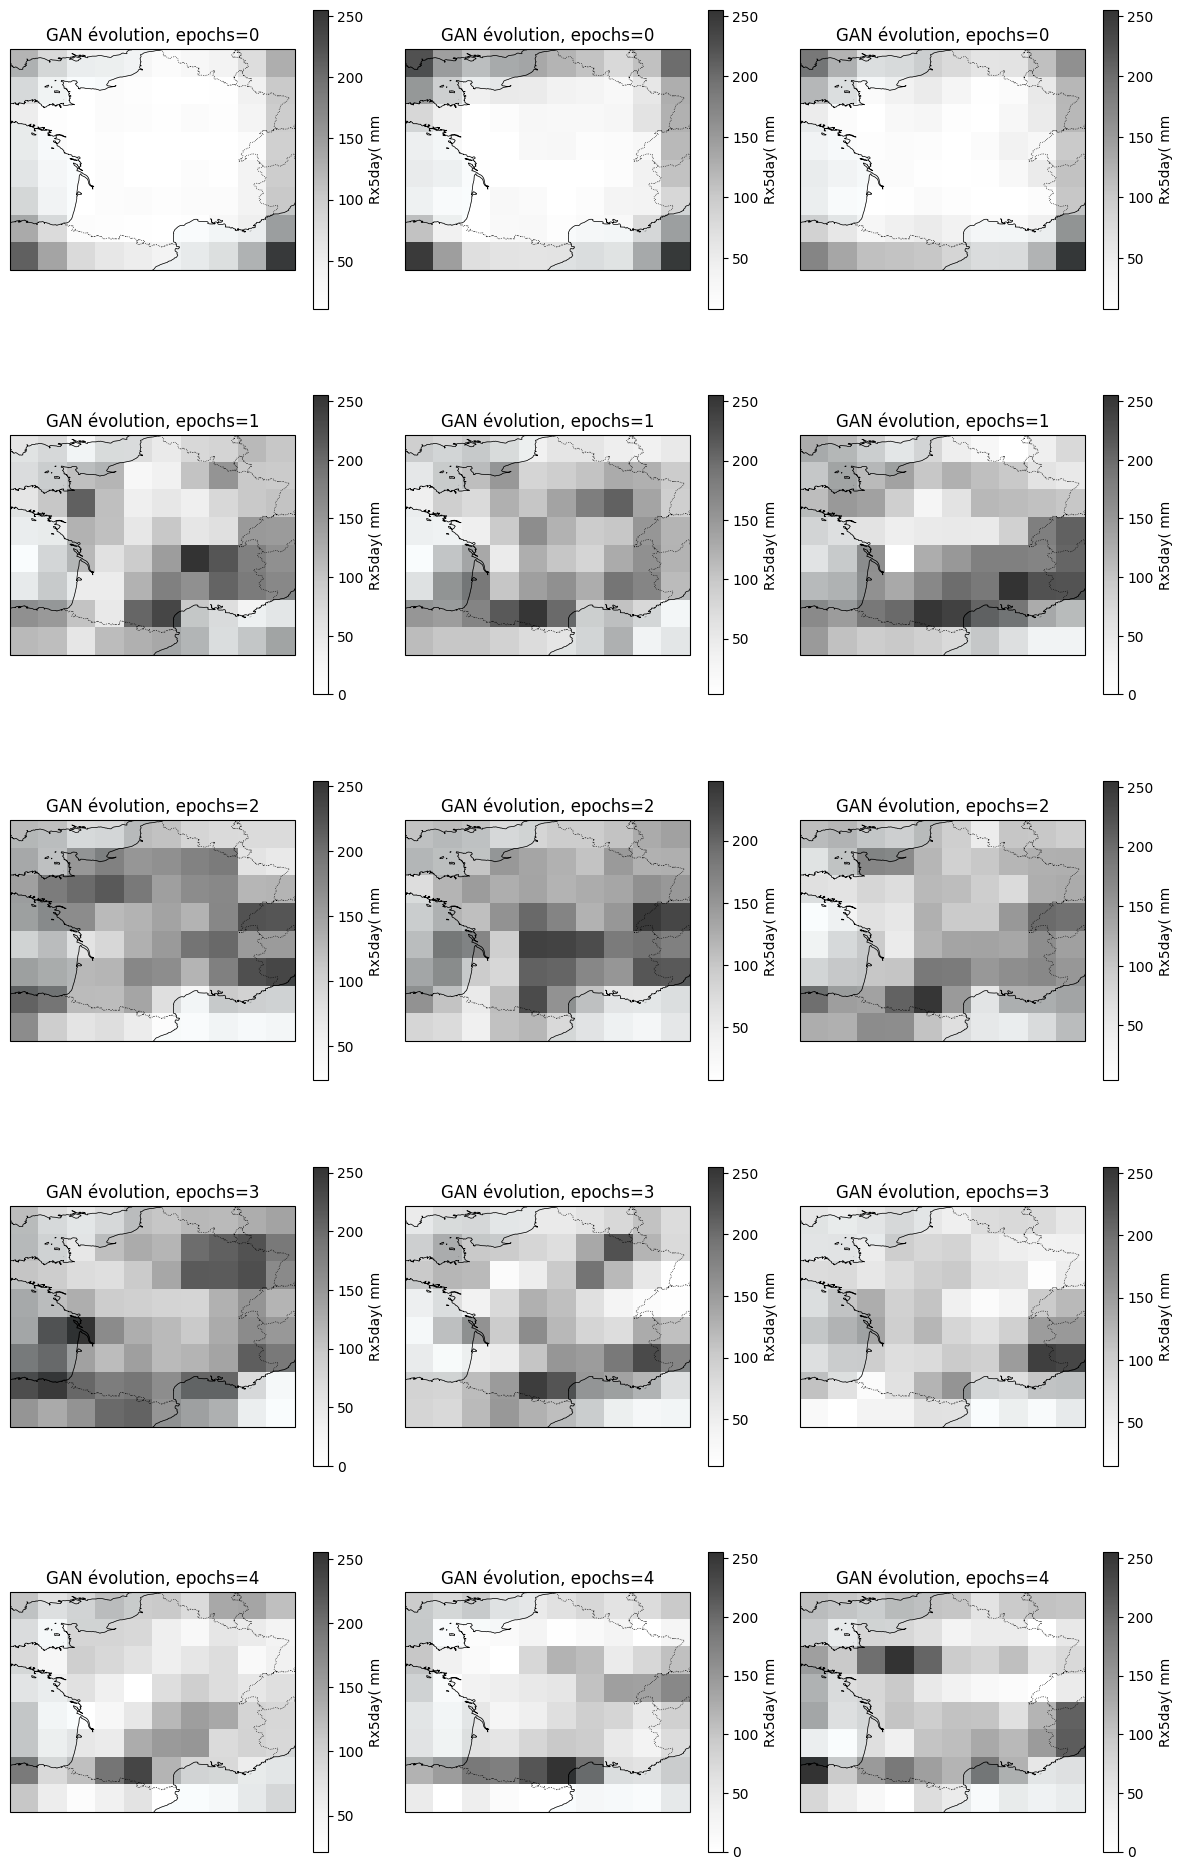
\includegraphics[width=0.82\textwidth]{../images/GAN/gan_generated_samples_over_epochs.png}
    \caption{Évolution des échantillons générés par le GAN.}
\end{figure}

\begin{figure}[H]
    \centering
    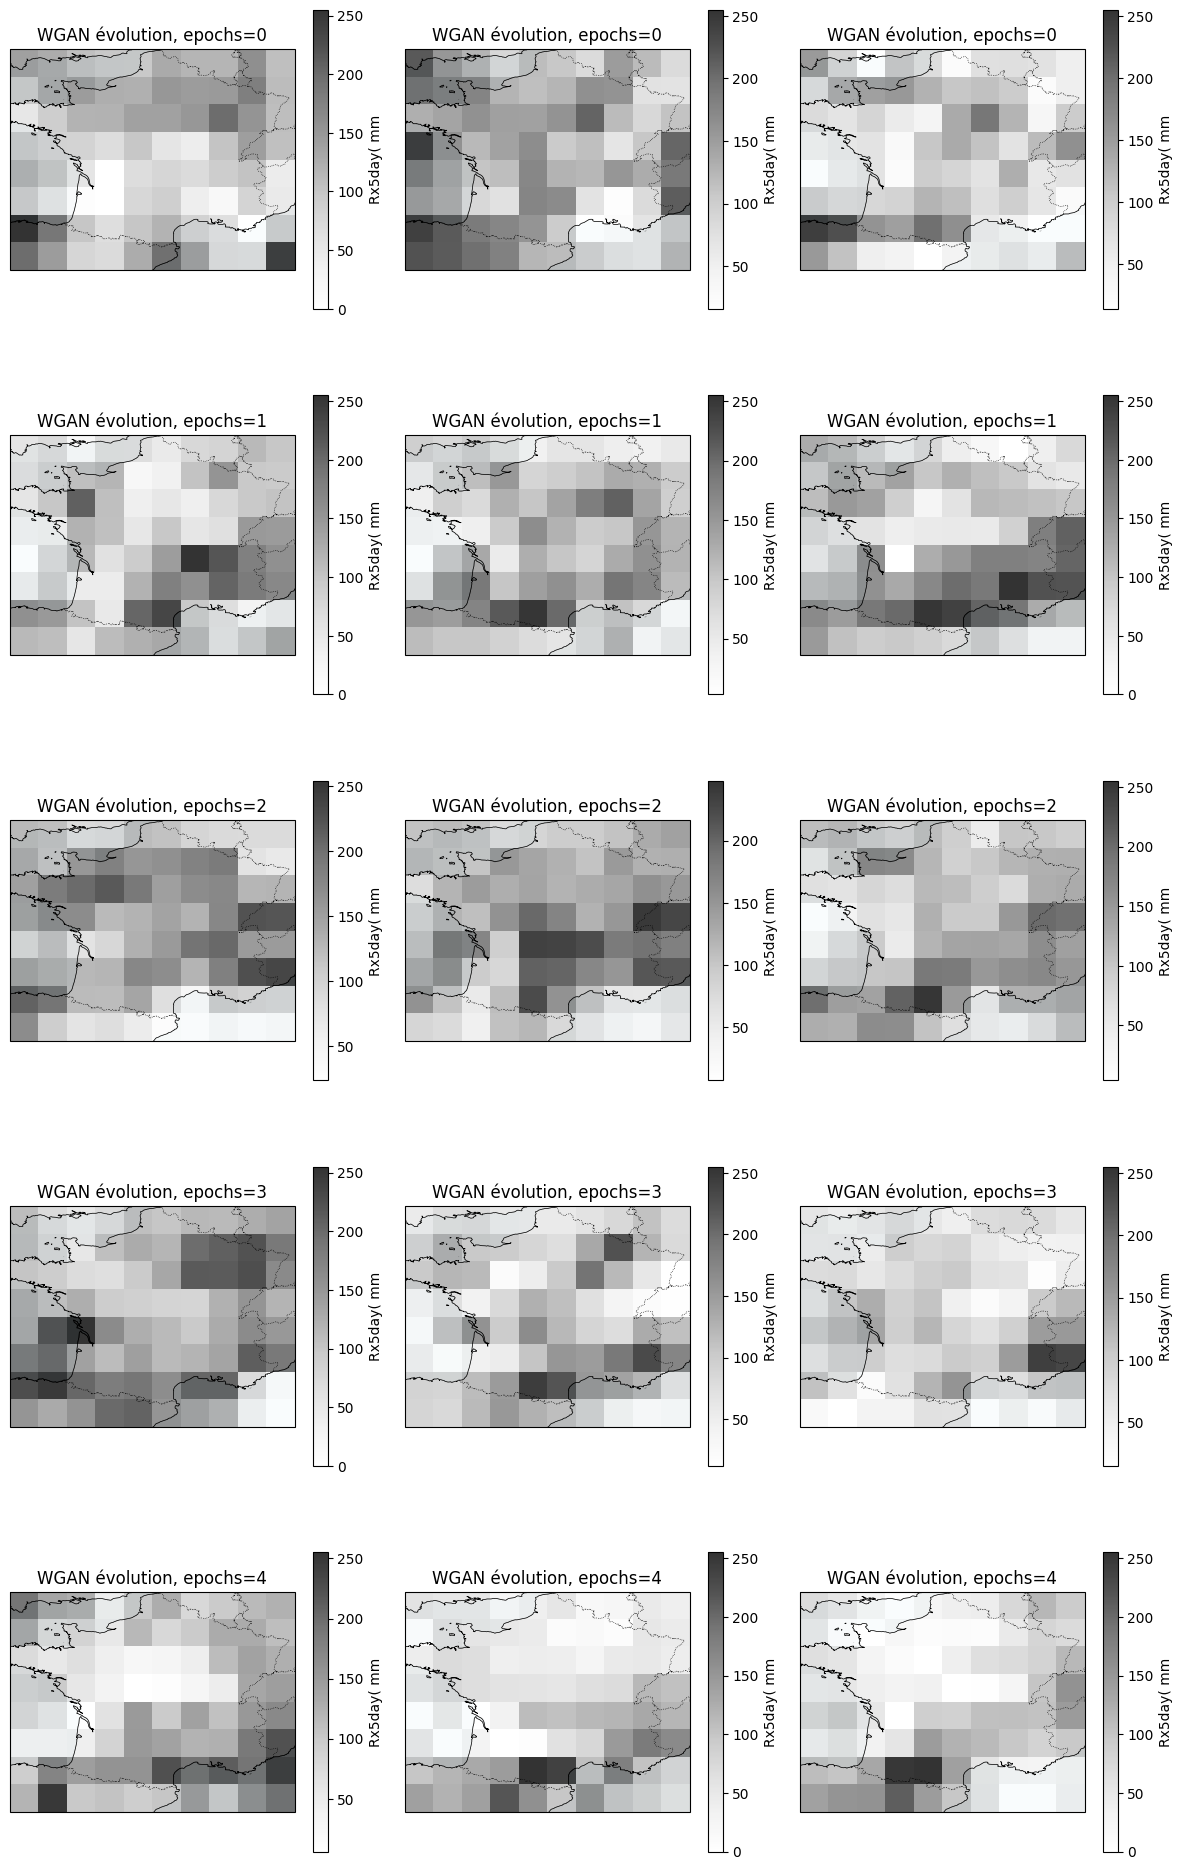
\includegraphics[width=0.82\textwidth]{../images/GAN/wgan_generated_samples_over_epochs.png}
    \caption{Évolution des échantillons générés par le WGAN-GP.}
\end{figure}

\end{document}
